\documentclass{beamer}
\usepackage{cmap}
\usepackage[utf8]{inputenc}
\usepackage[russian]{babel}
\usepackage{listings}
\usetheme{Antibes}
\usecolortheme{beaver}
\usepackage{graphicx}
\graphicspath{{img/}}

\title{Crowdsourcing morphological annotation in OpenCorpora project}
\author{Bocharov~Victor, Alexeeva Svetlana, Granovsky Dmitry,\\Stepanova Maria, Ostapuk Natalia\\\small\it OpenCorpora.org}
\date{31st~of~May 2012}
\begin{document}

% title page
\maketitle

%slide 01
\begin{frame}
\frametitle{OpenCorpora Project Summary}
\begin{enumerate}
\item{Goals}
    \begin{itemize}
    \item{corpus for machine learning tasks}
    \item{available under free license}
    \item{with deep manual annotation}
    \end{itemize}
    \pause
\item{Restrictions}
    \begin{itemize}
    \item{small because manual annotation takes a lot of time}
    \item{not well balanced due to license restrictions}
    \end{itemize}
    \pause
\item{Current State}
    \begin{itemize}
    \item{680K of words}
    \item{manual tokenization}
    \item{manual sentece boundaries}
    \item{morphological annotation just started}
    \end{itemize}
\end{enumerate}
\end{frame}

%slide 02
\begin{frame}
\frametitle{Morphological annotation}
\begin{enumerate}
\item{Automatic, dictionary-based}
    \begin{itemize}
    \item{dictionary - AOT (www.aot.ru)}
    \item{about 2.6 homonyms per word}
    \end{itemize}
\item{Manual disambiguation}
    \begin{itemize}
    \item{marking right / wrong hypotheses}
    \item{partial disambiguation allowed}
    \item{done by volunteers}
    \end{itemize}
\end{enumerate}
\end{frame}

%slide 03
\begin{frame}
\frametitle{Dictionary-based morphological annotation}
\begin{figure}
\center{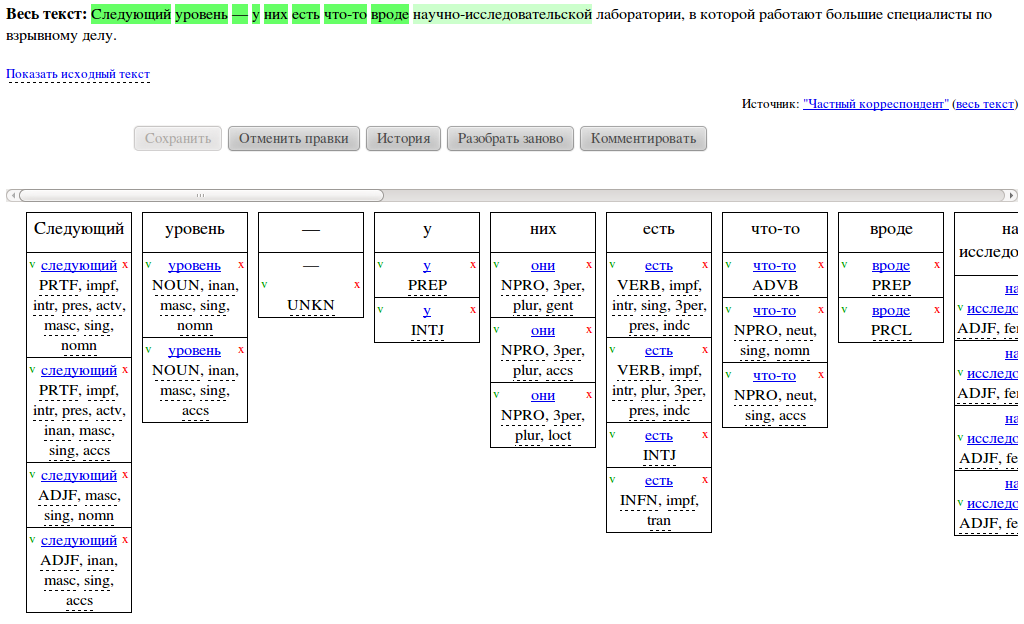
\includegraphics[width=1\linewidth]{2012_miem_5.png}}
\end{figure}
\end{frame}


%slide 04
\begin{frame}
\frametitle{Morphological annotation}
\begin{enumerate}
\item{Challenges}
    \begin{itemize}
    \item{Takes a lot of time}
    \item{Requires qualified annotators}
    \item{Everybody makes mistakes}
    \end{itemize}
    \pause
\item{Solutions}
    \begin{itemize}
    \item{annotation is splitted into simple annotation tasks}
        \begin{itemize}
        \item{"... выпуски ПРОГРАММЫ обходились ..." - singular or plural?}
        \item{"Этот НАСТРОЙ распространился ..." - noun or verb?}
        \end{itemize}
    \item{annotation tasks are grouped per question type}
    \item{all tasks are given to several annotators}
    \item{answers are verified}
    \end{itemize}
\end{enumerate}
\end{frame}

%slide 05
\begin{frame}
\frametitle{Annotation life cycle}
\begin{figure}
\center{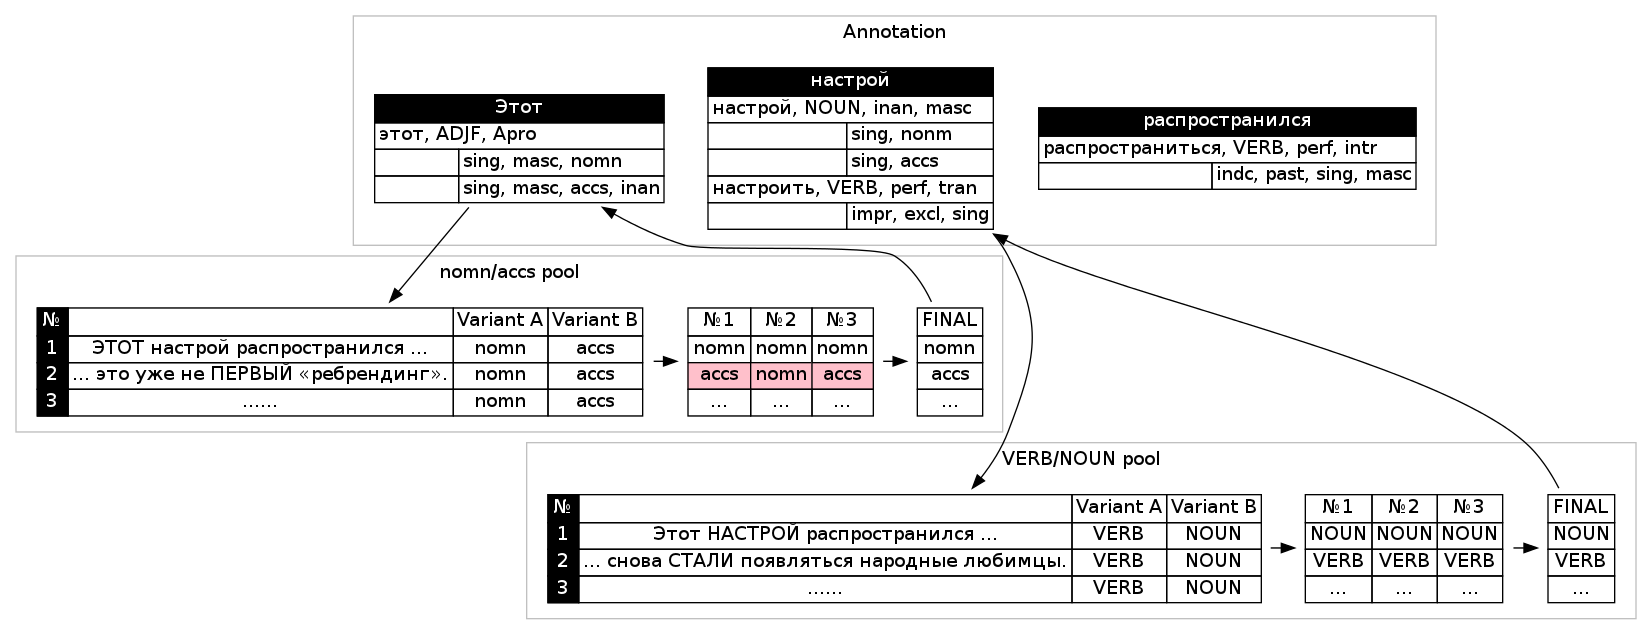
\includegraphics[width=1\linewidth]{annotation-lifecycle.png}}
\end{figure}
\end{frame}


%slide 06
\begin{frame}
\frametitle{Annotation interface}
\begin{figure}
\center{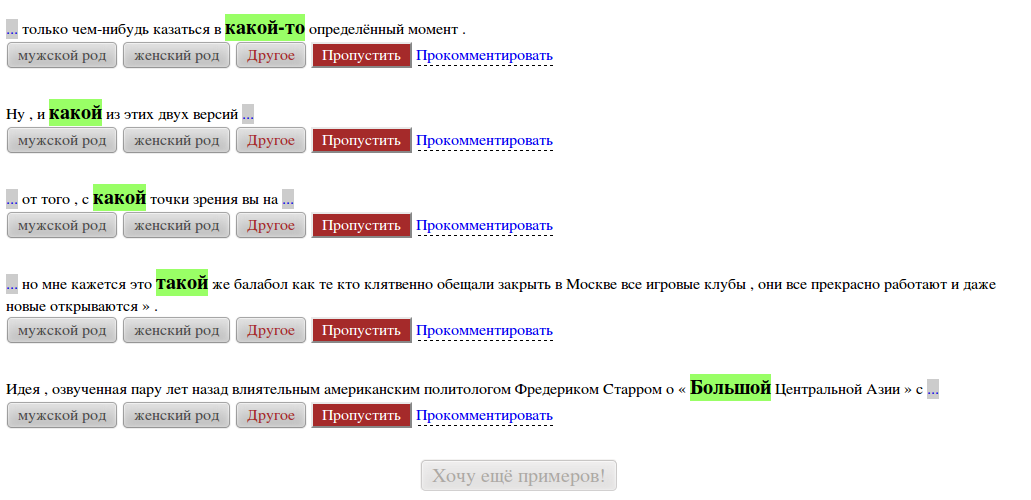
\includegraphics[width=1\linewidth]{2012_miem_4.png}}
\end{figure}
\end{frame}

%slide 07
\begin{frame}
\frametitle{Verification interface}
\begin{figure}
\center{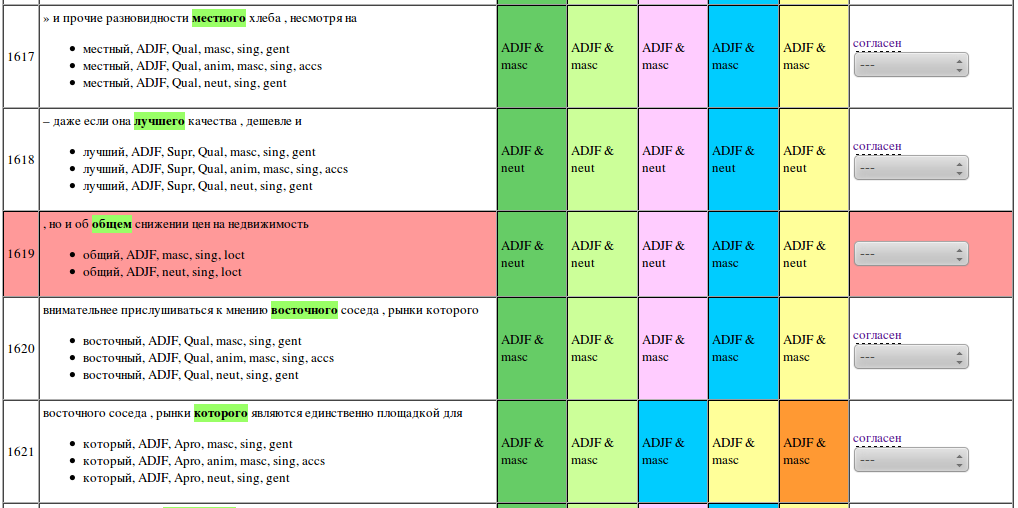
\includegraphics[width=1\linewidth]{2012_miem_6.png}}
\end{figure}
\end{frame}


%slide 08
\begin{frame}
\frametitle{Live demonstration}
\begin{enumerate}
\item{Sign up at http://opencorpora.org}
    \begin{itemize}
    \item{Accept license CC-BY-SA}
    \end{itemize}
\item{Choose annotation pool}
\item{Do annotation until tired}
\end{enumerate}
\end{frame}

%slide 09
\begin{frame}
Questions?
\end{frame}

%slide 09 
\begin{frame}
\frametitle{Contacts}
\begin{center}
\LARGE http://opencorpora.org\\[\bigskipamount]
\Large\texttt{opencorpora@opencorpora.org}
\end{center}
\end{frame}

\end{document}
